\title{CS378 Architecture: \\ Homework 3 Report}
\author{Rushi Shah}
\date{\today}

\documentclass{article}
\usepackage{graphicx}
\usepackage{url}
\usepackage[margin=1.2in]{geometry}

\begin{document}
\maketitle



\section{Experiments}

I tracked global branch histories and plugged them into a Linear Support Vector Classification from sklearn. I tracked histories of length 16, 32, and 64. I also experimented with hyper-parameter tuning of the penalty parameter with $C = 1, 1^{-2}, 1^{-4}, 1^{-8}$. The experiments were evaluated with the \texttt{cross\_validate} function implemented in the sklearn library to separate training data from testing data.   

\section{Results}

Scroll to the bottom of the report to see the graphs. 

\section{Conclusions}

\subsection{Penalty Parameters}

In astar and bzip there is a threshold below which the penalty parameter seems to start destroying performance. This can be seen most clearly in the first graph where the purple bar for $C = 1^{-8}$ is significantly lower than the other three bars. However, this phenomenon is not observed in other benchmarks, where the penalty parameter seems to have negligible effects on overall performance. 

\subsection{History Length}

Longer history lengths clearly correlate with higher accuracy in the astar benchmark. This can be most clearly seen in the first set of bars in the second graph, which follow a nice upward slope as history length goes from 16 to 64. However, in other benchmarks it seems that the higher history lengths do not contribute to performance because the red, blue, and green bars are roughly equal regardless of history length. This is an important observation because lower history lengths require less hardware overhead to track. 


\pagebreak

\begin{figure}[t]
  \centering
  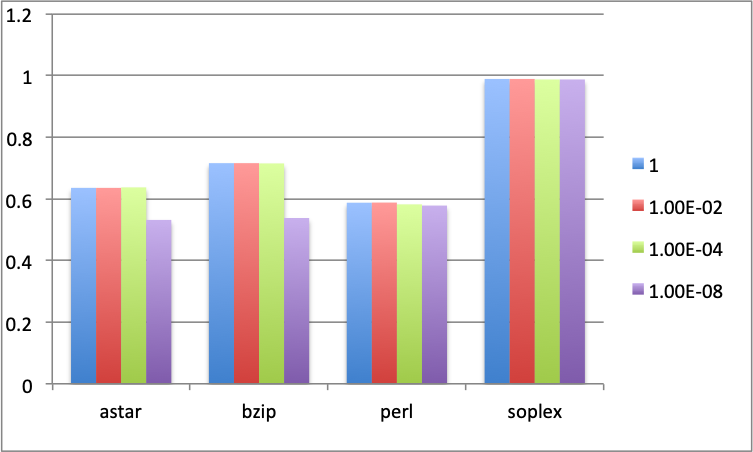
\includegraphics[width=.75\textwidth]{penalty-param.png}
  \caption{Accuracy as compared to the penalty parameter.}
\end{figure}

\begin{figure}[t]
  \centering
  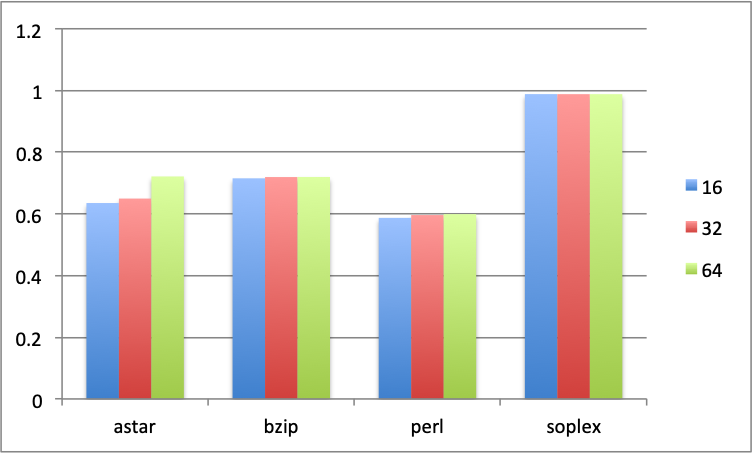
\includegraphics[width=.75\textwidth]{history-length.png}
  \caption{Accuracy as compared to the history length.}
\end{figure}

% \begin{figure}[t]
%   \centering
%   % 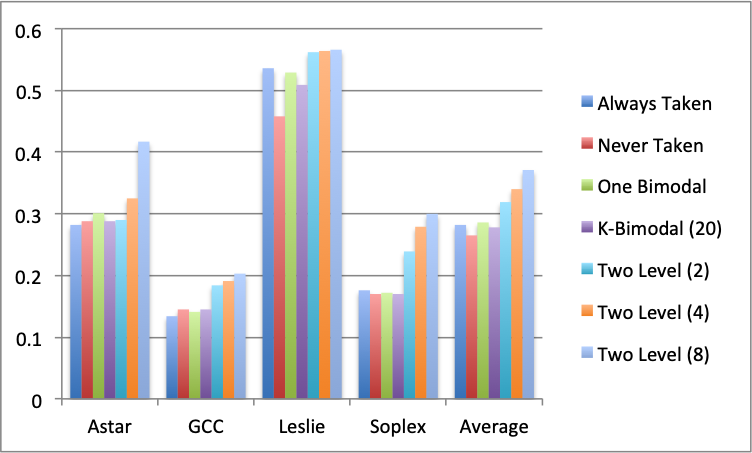
\includegraphics[height=.45\textheight]{ipc.png}
%   \caption{Branch Predictor Accuracy.}
% \end{figure}


\end{document}